%license:BSD-3-Clause
%copyright-holders:Michele Maione
%============================================================
%
%	Piattaforma di cloud gaming per giochi arcade
%
%============================================================
\chapter{Implementazione}
%In questa sezione si spiega come è stato affrontato il problema concettualmente, la soluzione logica che ne è seguita senza la documentazione.
%Si mostra il progetto dell’architettura del sistema con i vari moduli.
In questo capitolo verranno descritte le cinque fasi aggiuntive del cloud gaming e la loro implementazione in C++ come nuovi moduli del MAME: la cattura audio-video, la codifica, la trasmissione, la decodifica e la gestione dell'input utente.




\section{Cattura}
Lorem ipsum dolor sit amet, consectetur adipiscing elit, sed do eiusmod tempor incididunt ut labore et dolore magna aliqua. Ut enim ad minim veniam, quis nostrud exercitation ullamco laboris nisi ut aliquip ex ea commodo consequat. Duis aute irure dolor in reprehenderit in voluptate velit esse cillum dolore eu fugiat nulla pariatur. Excepteur sint occaecat cupidatat non proident, sunt in culpa qui officia deserunt mollit anim id est laborum.

Lorem ipsum dolor sit amet, consectetur adipiscing elit, sed do eiusmod tempor incididunt ut labore et dolore magna aliqua. Ut enim ad minim veniam, quis nostrud exercitation ullamco laboris nisi ut aliquip ex ea commodo consequat. Duis aute irure dolor in reprehenderit in voluptate velit esse cillum dolore eu fugiat nulla pariatur. Excepteur sint occaecat cupidatat non proident, sunt in culpa qui officia deserunt mollit anim id est laborum.


\subsection{Video}
Le funzioni della libreria SDL utilizzate sono:

\begin{itemize}
	\item CreateRGBSurfaceWithFormat: Crea una superficie RGB specificando il formato pixel da utilizzare;
	\item CreateRenderer: Crea un contesto di rendering 2D per una finestra;
	\item CreateSoftwareRenderer: Crea un contesto di rendering 2D per una superficie;
	\item RWFromMem: Prepara un buffer di memoria di lettura-scrittura da utilizzare con la struttura dati RWops (read-write opaque pointer structure);
	\item SetRenderDrawColor: Imposta il colore utilizzato per le operazioni di disegno;
	\item RenderFillRect: Riempe un rettangolo con il colore di disegno corrente;
	\item RenderDrawLine: Disegna una linea con il colore di disegno corrente;
	\item RenderPresent: Aggiorna il contesto di rendering con il frame generato dalle funzioni di disegno.
\end{itemize}

\begin{figure}[H]
	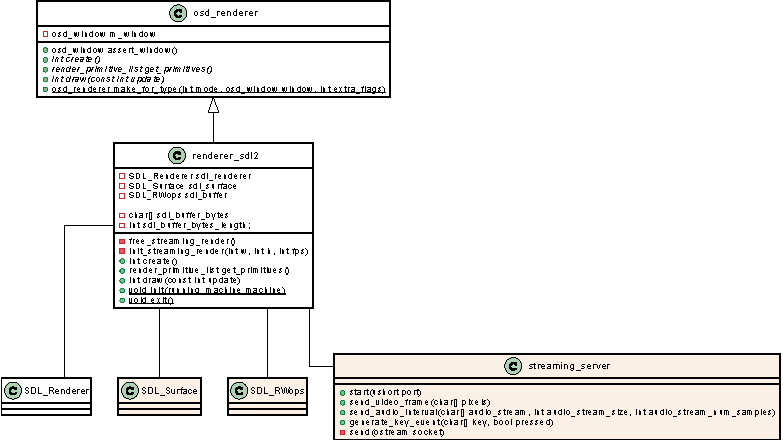
\includegraphics[width=\linewidth]{immagini/render_class_original_vs_streaming}
	\caption{Diagramma delle classi (parziale) relative al rendering}
	\label{fig:render_class_original_vs_streaming}
\end{figure}


\subsection{Audio} \label{Cattura_Audio}
Lorem ipsum dolor sit amet, consectetur adipiscing elit, sed do eiusmod tempor incididunt ut labore et dolore magna aliqua. Ut enim ad minim veniam, quis nostrud exercitation ullamco laboris nisi ut aliquip ex ea commodo consequat. Duis aute irure dolor in reprehenderit in voluptate velit esse cillum dolore eu fugiat nulla pariatur. Excepteur sint occaecat cupidatat non proident, sunt in culpa qui officia deserunt mollit anim id est laborum.




\section{Codifica}
Lorem ipsum dolor sit amet, consectetur adipiscing elit, sed do eiusmod tempor incididunt ut labore et dolore magna aliqua. Ut enim ad minim veniam, quis nostrud exercitation ullamco laboris nisi ut aliquip ex ea commodo consequat. Duis aute irure dolor in reprehenderit in voluptate velit esse cillum dolore eu fugiat nulla pariatur. Excepteur sint occaecat cupidatat non proident, sunt in culpa qui officia deserunt mollit anim id est laborum.

\subsection{MPEG}
Lorem ipsum dolor sit amet, consectetur adipiscing elit, sed do eiusmod tempor incididunt ut labore et dolore magna aliqua. Ut enim ad minim veniam, quis nostrud exercitation ullamco laboris nisi ut aliquip ex ea commodo consequat. Duis aute irure dolor in reprehenderit in voluptate velit esse cillum dolore eu fugiat nulla pariatur. Excepteur sint occaecat cupidatat non proident, sunt in culpa qui officia deserunt mollit anim id est laborum.

\subsubsection{Compression}
Lorem ipsum dolor sit amet, consectetur adipiscing elit, sed do eiusmod tempor incididunt ut labore et dolore magna aliqua. Ut enim ad minim veniam, quis nostrud exercitation ullamco laboris nisi ut aliquip ex ea commodo consequat. Duis aute irure dolor in reprehenderit in voluptate velit esse cillum dolore eu fugiat nulla pariatur. Excepteur sint occaecat cupidatat non proident, sunt in culpa qui officia deserunt mollit anim id est laborum.

\subsubsection{Video}
Lorem ipsum dolor sit amet, consectetur adipiscing elit, sed do eiusmod tempor incididunt ut labore et dolore magna aliqua. Ut enim ad minim veniam, quis nostrud exercitation ullamco laboris nisi ut aliquip ex ea commodo consequat. Duis aute irure dolor in reprehenderit in voluptate velit esse cillum dolore eu fugiat nulla pariatur. Excepteur sint occaecat cupidatat non proident, sunt in culpa qui officia deserunt mollit anim id est laborum.

\subsubsection{Audio}
Lorem ipsum dolor sit amet, consectetur adipiscing elit, sed do eiusmod tempor incididunt ut labore et dolore magna aliqua. Ut enim ad minim veniam, quis nostrud exercitation ullamco laboris nisi ut aliquip ex ea commodo consequat. Duis aute irure dolor in reprehenderit in voluptate velit esse cillum dolore eu fugiat nulla pariatur. Excepteur sint occaecat cupidatat non proident, sunt in culpa qui officia deserunt mollit anim id est laborum.

\subsubsection{Trasmission}
Lorem ipsum dolor sit amet, consectetur adipiscing elit, sed do eiusmod tempor incididunt ut labore et dolore magna aliqua. Ut enim ad minim veniam, quis nostrud exercitation ullamco laboris nisi ut aliquip ex ea commodo consequat. Duis aute irure dolor in reprehenderit in voluptate velit esse cillum dolore eu fugiat nulla pariatur. Excepteur sint occaecat cupidatat non proident, sunt in culpa qui officia deserunt mollit anim id est laborum.

\subsection{FFmpeg}
Lorem ipsum dolor sit amet, consectetur adipiscing elit, sed do eiusmod tempor incididunt ut labore et dolore magna aliqua. Ut enim ad minim veniam, quis nostrud exercitation ullamco laboris nisi ut aliquip ex ea commodo consequat. Duis aute irure dolor in reprehenderit in voluptate velit esse cillum dolore eu fugiat nulla pariatur. Excepteur sint occaecat cupidatat non proident, sunt in culpa qui officia deserunt mollit anim id est laborum \parencite{FFmpeg_Documentation}.

\subsubsection{Libs.}
Lorem ipsum dolor sit amet, consectetur adipiscing elit, sed do eiusmod tempor incididunt ut labore et dolore magna aliqua. Ut enim ad minim veniam, quis nostrud exercitation ullamco laboris nisi ut aliquip ex ea commodo consequat. Duis aute irure dolor in reprehenderit in voluptate velit esse cillum dolore eu fugiat nulla pariatur. Excepteur sint occaecat cupidatat non proident, sunt in culpa qui officia deserunt mollit anim id est laborum.




\section{Trasmissione}
Lorem ipsum dolor sit amet, consectetur adipiscing elit, sed do eiusmod tempor incididunt ut labore et dolore magna aliqua. Ut enim ad minim veniam, quis nostrud exercitation ullamco laboris nisi ut aliquip ex ea commodo consequat. Duis aute irure dolor in reprehenderit in voluptate velit esse cillum dolore eu fugiat nulla pariatur. Excepteur sint occaecat cupidatat non proident, sunt in culpa qui officia deserunt mollit anim id est laborum.

\subsection{Web APIs}
Le API Web sono un insieme di API e interfacce che comprendono la potente capacità di creazione di script del Web. A seguire quelli utilizzati in questo progetto \parencite{Web_APIs}.

\subsubsection{WebSocket}
WebSocket è un protocollo di comunicazione del computer che fornisce canali di comunicazione full-duplex su una singola connessione TCP. È compatibile con HTTP perché l'handshake WebSocket utilizza l'intestazione di aggiornamento HTTP per passare dal protocollo HTTP al protocollo WebSocket. È supportato nativamente da tutti i browser e il suo utilizzo è simile ai normali socket sia sul lato client che su quello server. Per questi motivi è il protocollo di comunicazione generico più utilizzato sul web \parencite{WebSocket_Web_APIs}.




\section{Decodifica}
Lorem ipsum dolor sit amet, consectetur adipiscing elit, sed do eiusmod tempor incididunt ut labore et dolore magna aliqua. Ut enim ad minim veniam, quis nostrud exercitation ullamco laboris nisi ut aliquip ex ea commodo consequat. Duis aute irure dolor in reprehenderit in voluptate velit esse cillum dolore eu fugiat nulla pariatur. Excepteur sint occaecat cupidatat non proident, sunt in culpa qui officia deserunt mollit anim id est laborum.

\subsection{Web APIs}
Le API Web sono un insieme di API e interfacce che comprendono la potente capacità di creazione di script del Web. A seguire quelli utilizzati in questo progetto \parencite{Web_APIs}.

\subsubsection{Canvas API}
L'API Canvas fornisce un mezzo per disegnare grafica tramite JavaScript, si concentra principalmente sulla grafica 2D ma quando viene utilizzata dall'API WebGL può disegnare grafica 2D e 3D con accelerazione hardware. È completamente supportato da tutti i browser \parencite{Canvas_API}.

\subsubsection{WebGL API}
WebGL è un'API JavaScript, progettata e gestita dal gruppo no-profit Khronos, per il rendering di grafica 2D e 3D che consente l'utilizzo accelerato dalla GPU della fisica e dell'elaborazione e degli effetti delle immagini. WebGL 1.0 è supportato su tutti i browser, mentre WebGL 2.0 viene testato su Safari \parencite{WebGL}.



\subsection{Librerie JavaScript}
Per il front-end, sono state utilizzate una libreria JavaScript open source per la decodifica del filmato.

\subsubsection{JSMpeg}
JSMpeg è una libreria composta da un demuxer MPEG-TS, un decoder video MPEG1 e audio MP2, con un sistema di rendering basato sia su WebGL che su Canvas2D, ed un sistema di output audio basato su WebAudio. Consente lo streaming a bassa latenza ($\sim$50ms) tramite WebSocket, ed è rilasciata con licenza MIT \parencite{JSMpeg}.




\section{Gestione input}
Lorem ipsum dolor sit amet, consectetur adipiscing elit, sed do eiusmod tempor incididunt ut labore et dolore magna aliqua. Ut enim ad minim veniam, quis nostrud exercitation ullamco laboris nisi ut aliquip ex ea commodo consequat. Duis aute irure dolor in reprehenderit in voluptate velit esse cillum dolore eu fugiat nulla pariatur. Excepteur sint occaecat cupidatat non proident, sunt in culpa qui officia deserunt mollit anim id est laborum.

\subsection{Librerie JavaScript}
Per il front-end, sono state utilizzate due librerie JavaScript open source per la gestione degli input.

\subsubsection{Keypress}
Keypress è una libreria per la cattura dell'input da tastiera specializzata per l'uso in contesti videoludici, rilasciata con licenza Apache 2.0. Viene utilizzata per gestire l'input da tastiera nel front-end \parencite{Keypress}.

\subsubsection{GameController.js}
GameController.js è una libreria che estende le Web API per il gamepad, è rilasciata con licenza MIT. Nel front-end viene utilizzata per gestire i gamepads, per consentire il multiplayer sullo stesso dispositivo \parencite{gameController_js}.


\subsection{SDL input}
Lorem ipsum dolor sit amet, consectetur adipiscing elit, sed do eiusmod tempor incididunt ut labore et dolore magna aliqua. Ut enim ad minim veniam, quis nostrud exercitation ullamco laboris nisi ut aliquip ex ea commodo consequat. Duis aute irure dolor in reprehenderit in voluptate velit esse cillum dolore eu fugiat nulla pariatur. Excepteur sint occaecat cupidatat non proident, sunt in culpa qui officia deserunt mollit anim id est laborum.

%\parencite{CPP_Primer}
%\parencite{Computer_Networking_and_the_Internet}
%\parencite{Ingegneria_del_software}
%\parencite{Understanding_the_Linux_Kernel}
%\parencite{Windows_Server_2012}